\begin{section}{Evaluation of Activity Recognition}
	The main task of this work is dedicated to human activity recognition, which is a challenging task of current research. In the following sections we will present and discuss our performed experiments.
	\begin{subsection}{Reproduction and Baseline}
		In order to be able to compare our efforts to the results reported by the original paper, we first tried to recreate the classifier used by Vaizman et al. in initial paper of the dataset. They used logistic regression \ref{subsec:lr} as a baseline and reached a balanced accuracy of $0.718$ with instance-weighting and $0.598$ without \cite{Vaizman18}. Our method reaches an accuracy of $0.656$ without instance-weighting (see chapter \ref{sec:instance_weighting} for more details on instance weighting). There might be various reasons why our implementation performed better than the original. Differences in the implementation of the algorithm in different libraries may be one, as well as optimized hyper parameters. We used Bayesian Optimization (see chapter \ref{subsec:bayes_opt}) to search for mentioned hyperparameters. 
		We expanded our baseline by some more classical methods, including an Naive-Bayes-Classifier with Gaussian distribution for every feature. The results were slightly better than chance, with a balanced accuracy of $0.555$. This indicates that the assumptions made for Naive Bayes about the independence and normal distribution of each feature (see \ref{subsec:naive_bayes}) most likely does not hold. \par
		Before focusing on tree ensemble methods, we first experimented with a Linear Support Vector Machine (short LinSVC (\emph{C} for Classifier)). We did a hyperparameter search with Bayesian Optimization, but the resulting balanced accuracy of $0.636$ is below the results obtained by logistic regression. In addition, the implementation provided by Scikit-Learn does not support GPU's, resulting in very long training time. \par
	\end{subsection}

	\begin{subsection}{Random Forest and XGBoost}
		In a first attempt, we decided to have a use the classic Random Forest ensemble method (see chapter \ref{subsec:random_forests}). Analogous to our baseline algorithms, we tried to improve the results using Bayesian Optimization. This combination almost reproduced our results obtained by logistic regression already, achieving a balanced accuracy of $0.650$. We then decided to use a more sophisticated tree ensemble method, namely Gradient Tree Boosting (see chapter \ref{subsec:grad_boost}). The two most used implementations, XGBoost (see chapter \ref{subsec:xgb}) and LightGBM\footnote{\href{https://github.com/microsoft/LightGBM}{github.com/microsoft/LightGBM}} became widely recognized over the past years for their successes in many machine learning competitions \cite{Chen16}. \par
		We were able to improve the classification accuracy achieved by logistic regression and Random Forests using XGBoost slightly. After tuning the hyperparameters, again using Bayesian Optimization, the final balanced accuracy was $0.672$.  The following table summarizes our achieved scores, including the results for our Ensemble Classification approach (see chapter \ref{subsec:stacking}). All scores are calculated using 5-fold cross validation.
		\begin{table}[H]
			\begin{center} 
				\begin{tabular}{r|c|c}
					\toprule
					& Stratified & Grouped \\
					\midrule
					Logistic Regression & 0.809 & 0.656 \\
					Naive Bayes & 0.567 & 0.555 \\
					LinSVC & 0.780 & 0.636 \\
					Random Forest & 0.954 & 0.650 \\
					\textbf{XGBoost} & \textbf{0.958} & \textbf{0.672} \\
					\midrule
					Ensemble & 0.941 & \\
					\bottomrule
				\end{tabular}
			\end{center}
			\caption{Summary of classification results on the ExtraSensory Dataset. All values refer to balanced accuracy. Scores under \glqq Grouped\grqq{} refer to training with separated users (as done in the original paper). See chapter \ref{subsec:stratified} for additional information about results under \glqq Stratified\grqq.}
			\label{table:results}
		\end{table}
	\end{subsection}

	\begin{subsection}{Stacking}
		Stacking is a useful technique to combine the strengths of several different classifiers and compensate their weaknesses. It was proved to be successful in a variety of contexts and is the de facto state of the art in data science competitions without computer vision or natural language processing tasks.
		
		However, because of the computationally expensive internal cross validated training of prediction sets for the meta classifier, we need several good level one classifiers, that behave as differently as possible. Scikit-Learn offers a large variety of classifiers that follow different paradigms and differ in their strengths and weaknesses. The lack of GPU support is a major drawback of this library, particularly in a task where we need to train many classifiers at the same time for multi-activity recognition. We tested our algorithms on a modern personal computer with a twelve core Threadripper 2920x CPU, 64 GB of RAM and a nVidia RTX 2080 GPU.
		
		While a run of \texttt{FlexOneVsRestClassifier} with an 80/20 train-test-split takes about five minutes, resulting in 25 minutes for five fold  cross-validation, our tests with Scikit-Learn's \texttt{LinearSVC}, that is based on the efficient \texttt{liblinear} library, took more than 28 hours. Gaussian naive Bayes is a rather fast algorithm, but its accuracy was not high. The AdaBoost run time for training a single label was already were slow. As result we could not use it for the full multi-label problem in reasonable time. In the end, we were left with Scikit-Learn's logistic regression and the fast GPU implementations of XGBoost's gradient boosted trees and random forest.
		
		The stacking architecture we finally used was the combination of these three models as first-level classifiers with another gradient boosted tree as meta classifier. A run of five fold cross-validation takes about five hours and the runtime is heavily dominated by the logistic regression. Using only three classifiers proved to be too few to exploit the benefits of the stacking architecture. The final balanced accuracy was not improved compared to those of the XGBoost-only approach, but a much longer runtime was required (see table \ref{table:results}). We conclude stacking is only advantageous, if a larger set of sufficiently good classifiers are available and can be trained quickly. For this reason we do not use stacking in our final classifier, but rather rely on XGBoost as single model.
	\end{subsection}

	\begin{subsection}{Activity Recognition with Mixed Data Split}\label{subsec:stratified}
		Following the original paper, the dataset is split into training and test subsets such that each user is contained entirely within one of the two subsets. That means each trained classifier is tested on samples provided by users that were not trained. We refer to this method of splitting as \glqq grouped\grqq{}. The orthogonal approach is to split the samples of each user evenly between the training and test set. More precisely, if for example 80\% of the entire data set is used to train, 80\% of the samples of \emph{each} user is contained within the training set, the other 20\% in the test set. We refer to this splitting method as \glqq stratified\grqq{}. \par
		Using a stratified split instead of the original grouped split, we were able to produce substantially better classification results throughout all used classifiers. The only exception is the Naive Bayes classifier, which only improved very slightly, reaching a balanced accuracy of $0.567$. \par
		A valid reason for this improvement - or rather why classification with a grouped split is such a difficult task - can be found by analyzing at the results of our user classification (see chapter \ref{sec:user_classification}). We are able to identify the correct user for a given sample within more than 99\% accuracy. This indicates each user is unique and distinguishable in terms of samples he or she provides. This implies on the other hand that it is very difficult to gain good insight about some user's activities when he or she is unknown to the classifier. This assumption is encouraged by the fact that our classification results for human activity recognition with grouped splits were really good when tested on its own training data. The average XGBoost classifier achieves a balanced accuracy of $0.98$ on its training dataset. 
	\end{subsection}
	
	\subsection{Evaluation Instance Weighting} \label{sec:instance_weighting}
	
	Some papers report instance weighting as one major method to improve the balanced accuracy score of a trained model. Consequently, we attempted to reproduce these results. We conducted 5-fold cross evaluation on the provided features of the entire ExtraSensory dataset with and without instance weighting. For reasons of comparison and to determine the best of our implemented classifiers, this was done for random forest, XGBoost, logistic regression and naive bayes classifiers. 
	
	We were not able to reproduce the improvements reported in literature (\cite{Vaizman18}, \cite{Saeed18}). Instead each classifier lost about 5-8 percent points in accuracy. In the following we discuss which sources of failure might be excluded and a possible explanations of the behavior.
	 
	The first obvious possible source of failure can be found in bad implementation. We are convinced that this is not the case for the following reasons: First of all if the data handling would be wrong there should be an effect on all experiments. This was not observed. Secondly we trained different models utilizing different API's. Since the error was not only observed for just one or a subset of the API's, we can consequently assume that the implementations of the classifiers are correct. Otherwise the error would be spreaded very far and should have been noticed by members of the large community using these API's. One additional possibility is a bad implementation of the weighting itself. As weighting function we used the count of the opposite label value divided by the count of the current label value. This a fairly simple implementation and was double checked. Therefore we assume our implementation to be correct. 
	
	The second possible source of the accuracy loss is an issue with the dataset itself. We refer to the highly unbalanced representations of true and false example for many labels already discussed in the dataset introduction. One example is the elevator label with just 200 positive, but 70996 negative labels. The quotient of negative to positive value counts is almost 355. While this is the worst case example there are many labels with a instance weighting above 50, thus drastically increasing the influence of these underrepresented positive and also some negative label on the training process. If the few labels do not, and most likely will not, provide a sufficient representation of the labels, a representative model can not be trained which in turn can not provide a good classification for those labels. In addition, the model is trained to an increasing false positive or false negative rate, because the tolerance towards those representatives is pushed.
	
	To prevent this overboosting we tested regulating the used weights of the instance weighting by reducing the growth rate. This was done by applying the square root function. In fact, the regularization did reduce the accuracy loss by about 3 percent points, but still an consistent decrease in balanced accuracy was observed. This theory could not be proven or disproved by us due to limited research time and remains an interesting challenge for future research. Furthermore this problem should not be the only influence, since Vaizman et al. performed very similar experiments with the same dataset seemingly contradicting our findings.
	
	
\begin{subsection}{Interpretability}
	
	One of the tasks for the project was to highlight the influence of the individual features on the classification result for the resulting final classifier.
	
	The library XGBoost, which was used to construct our final classifier, provides an answer to the question with the method \texttt{xgboost.plot\_importance}. In Fig. \ref{abb:feature_importance} we show an example of the output for the label 'at\_a\_bar'. It shows the F-score (frequency) for the features that were used most frequently as split features in the gradient trees involved.
	  
	
	\begin{figure}[H]
		\begin{center}
			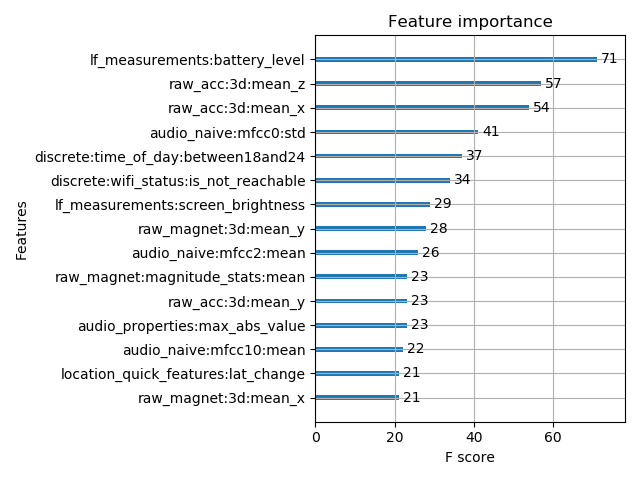
\includegraphics[width=.8\textwidth]{images/feature_importance.png}
			\caption{Shown are the 15 most frequent features which were involved assignment of the 'at\_a\_bar'}
			\label{abb:feature_importance}
		\end{center}		
	\end{figure}

    We have have to keep in mind: The usage-frequency of split-features is only \textit{somewhat} related to their importance, since the anti-overfitting measures limit the amount of total split and 'bad' splits are never included in the constructed trees. Then again the 'true' importance to the classification comes from the information gained by the splits, which is given by equation \ref{eq:LRsplit}. More frequent split-features have more $\LL_\text{split}$-values, but this fact does not indicate that the sum of those $\LL_\text{split}$-values is big. For example, there might be a binary feature like gender with a very high gain-value, but due to its structure it can only be used once and therefore has a low frequency-score.
    
    Therefore, statements derived from \texttt{xgboost.plot\_importance} are only conditionally meaningful.

\end{subsection}	
	
	\begin{subsection}{Future Directions}
		While trying to recreate results from both the original paper considering instance weighting (\cite{Vaizman18}) and Maximal Correlation Embedding by Li et al. (\cite{Li19}), we ran into some implementation problems. Naturally, these could be addressed in a future work and tried to be fixed, since the results reported by the underlying papers promise considerable improvement. \par
		A promising direction of future work could focus on establishing a greater and more effective ensemble classification architecture. Due to rather restrictive limits in computational power, we could not test architectures with more than a few classifiers, but we assume that adding a greater amount of different and diverse classifiers could improve the results of an ensemble classification. In order to utilize provided computational power as much as possible, we would focus on GPU-supporting algorithms only. \par
		Another interesting aspect of our current stacking architecture is the way data is split in the cross validation for the first-level classifier. Currently, a stratified split is used, although we train to optimize on grouped splits. Changing the cross validation to grouped splits could improve the overall classification results. \par
		All work referenced and considered in this report is based upon the official dataset with about 200 extracted features. However, the raw data collected by the sensors is also available for download. Future work could focus on using this raw data, maybe even in combination with the provided features. This would require a substantial amount of computing power, since the raw sensory data contains several GBs of information, but could also be insightful.
		
	\end{subsection}
\end{section}
